\subsection{Some extreme cases about Tutte's theorem}
In our project we do not use 3-connected graph but graph whose interior faces are triangle. It is obvious that considering the king of graphs we used Tutte's theorem is verified because the fypothesis « All interior faces are tringle » is lighter than « 3-connected » hypothesis. So now we changed the hypothesis about the external polyhgon and the interior vertices in order to find out if the tutte's  is always verified.  

\subsubsection{Tutte's theorem and concave polygon}

In this section, we changed the hypothesis about the graph face. Now we consider a concave polygon face. Below is the illustration of a couterexample. 

\begin {figure}[H]
  \centering
  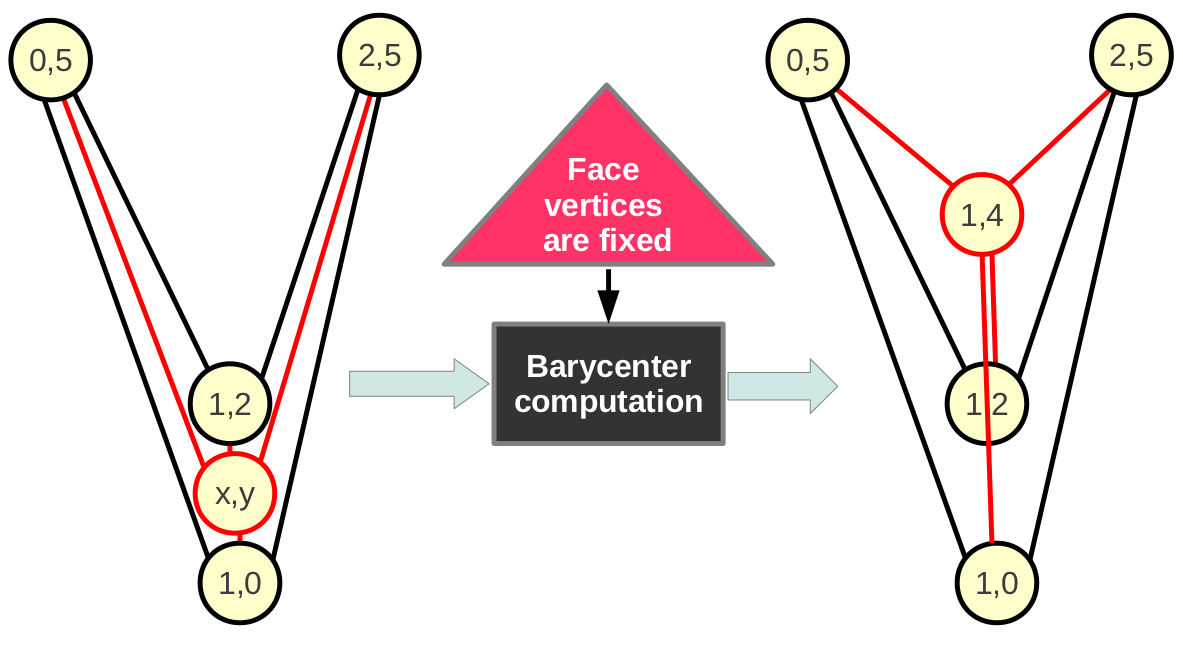
\includegraphics[scale=0.3]{img/tutte2.png}
  \caption{Tutte algorithm on concave polygon}
  \label{tutte2}
\end {figure}
\noindent
In the counterexample illustration above, the coordinate of the vertex shown in red color become $$(\frac{0+1+1+2}{4} , \frac{5+0+2+5}{4}) = (1 , 4)$$
One can see that after the the barycenter algorithm computation, the graph is no longer embedding. So the Tutte's theorem is not verified considering graphs with concave polygon face. 

\subsubsection{Tutte's algorithm and convex polygon with some fixed vertices}
This section kept the «convex polygon face» hypothesis but some internal vertices are considered fixed, their position never change during the barycenter algorithm computation. Below is the illustration of a couterexample. 

\begin {figure}[H]
  \centering
  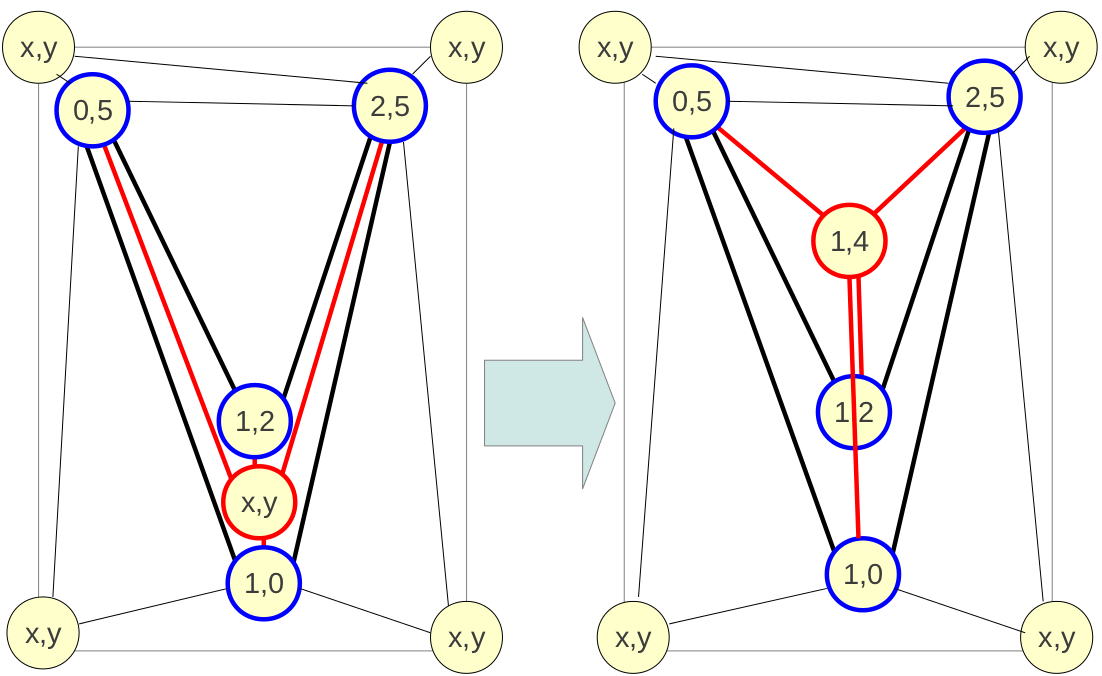
\includegraphics[scale=0.3]{img/tutte3.png}
  \caption{Tutte algorithm on convex polygon and fixes vertices}
  \label{tutte3}
\end {figure}
\noindent

As in the previous counterexample illustration (fig \ref{tutte2}) above, after the barycenter algorithm computation, the vertex shown in red color position changes. So the graph is no longer embedding which implies that the Tutte's theorem is not verified considering that some internal vertices can be fixed.
